\documentclass[a4paper,12pt]{report}

\usepackage{alltt, fancyvrb, url}
\usepackage{graphicx}
\usepackage[utf8]{inputenc}
\usepackage{hyperref}
\usepackage{array}
\usepackage[table]{xcolor}

% Questo commentalo se vuoi scrivere in inglese.
\usepackage[italian]{babel}

\usepackage[italian]{cleveref}

\title{Relazione per il progetto di\\``Programmazione di Reti''}

\author{Simone Rega \\ (0000915995)}
\date{\today}


\begin{document}
	
	\maketitle
	
	\tableofcontents
	
	\chapter{Introduzione}
	
	Il progetto consegnato rispecchia la Traccia 2 degli elaborati mostrati a lezione. 
	
	Il progetto si pone nello scenario di un insieme di device IoT, chiamati SmartMeter IoT, che mandano dati ad un Cloud Server, passando però prima da un Gateway si pone nel mezzo tra i due e ne gestisce le richieste.
	
	In questo progetto si farà uso di socket e di protocolli UDP e TCP.
	
	\chapter{Descrizione Architetturale}
	\subsection{IoT Devices}
	Gli SmartMeter IoT sono device che rilevano un numero ben definito di volte ogni giorno la temperatura e l'umidità del terreno in cui sono inseriti. 
	
	Questi Device si collegano una sola volta al giorno ad un Gateway per inviare le misure che hanno raccolto nelle 24 ore.
	
	Per questa connessione client-server viene utilizzato un protocollo UDP.
	
	\begin{figure}[!htb]
		\centering{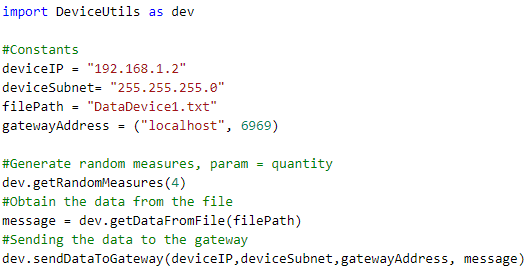
\includegraphics[width=\textwidth]{img/device.png}}
	\end{figure}
	
	I quattro client IoT sono stati realizzati separatamente \textit{(Device1.py, Device2.py, Device3.py, Device4.py)} i quali usufruiscono di due classi utility: DeviceUtils e AddressTools.
	
	Le funzioni principali di DeviceUtils sono:
	\begin{itemize}
		\item\textbf{ getRandomMeasures(quantity)}: dato un numero in ingresso che indica la quantità, la funzione provvederà a generare 4 file, o a sovrascriverli nel caso esistano già, e li popolerà con delle misure verosimili generate random.
		\item \textbf{getDataFromFile(filePath)}: dato un percorso di un file, la funzione procede ad aprire un file in lettura e leggerne il contenuto, restituendo una stringa in output contenente le rilevazioni.
		\item \textbf{sendToGateway(deviceIP,deviceSubnet,gatewayAddress, message}): la funzione crea un socket per una connessione UDP con il Gateway. Una volta stabilita la connessione viene inviato un pacchetto, tramite un buffer di 1024 Byte, contenente IP del device, Subnet Mask del device e il messaggio contente le misure rilevate.
	\end{itemize}

	Le funzioni principali di AddressTools sono:
	\begin{itemize}
		\item \textbf{getAddressEncoded}:restituisce l'indirizzo IP e la subnet mask contatenati e convertiti in byte, quindi in totale 16 Bytes.
		\item \textbf{convertBytesToIP(ipBytes, subnetBytes)}: dati in input un IP e una Subnet Mask in Bytes, la funzione si preoccupa di restituire un oggetto AddressTool contenente un ip e una subnet come stringhe.
	\end{itemize}

	\subsection{Gateway}
	Il Gateway fa da tramite tra i Device IoT e il Cloud Server. Prima si mette in ascolto sull'interfaccia di rete in cui ci sono i Device, attendendo che questi gli inviino i dati, per poi aprire una connessione TCP con il Cloud Server inviando tutte le rilevazioni ottenute dai vari Device.
	
	Il Gateway è stato realizzato nel modulo Gateway.py, usufruendo delle librerie socket e time.
	
	\begin{figure}[!htb]
		\centering{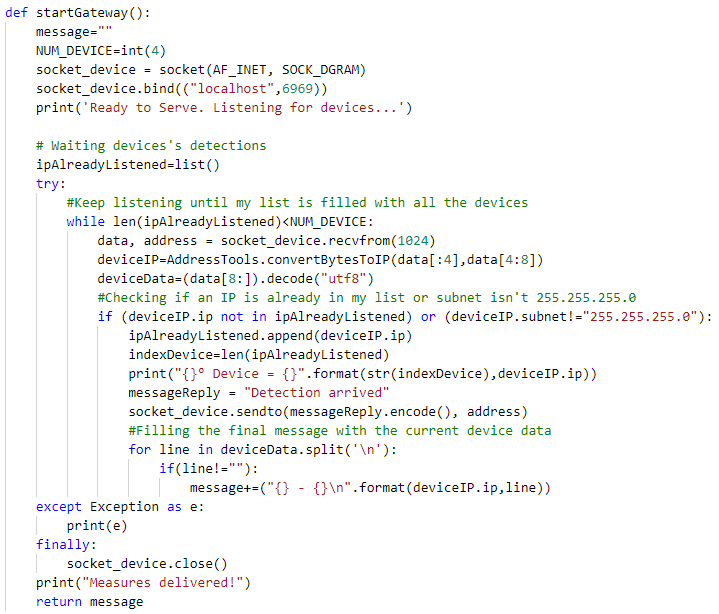
\includegraphics[width=\textwidth]{img/startgateway.png}}
		\caption{Metodo che fa partire il gateway e lo mette in ascolto dei socket IoT}
	\end{figure}

	\begin{figure}[!htb]
		\centering{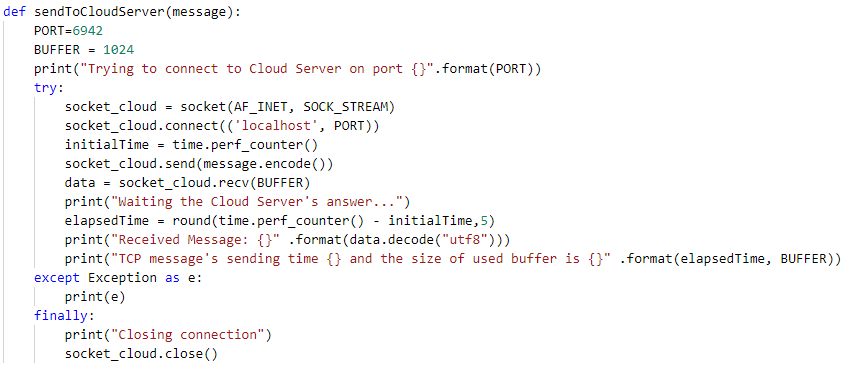
\includegraphics[width=\textwidth]{img/senttocloud.png}}
		\caption{Metodo che manda i dati al Cloud Server}
	\end{figure}	
	
	
	\subsection{Cloud Server}
	Il Cloud Server apre semplicemente una connessione TCP cpn il Gateway sull'interfaccia 10.10.10.0, mettendosi in ascolto e aspettando la ricezione del messaggio del Gateway contenente i dati delle rilevazioni.
	
	\begin{figure}[!htb]
		\centering{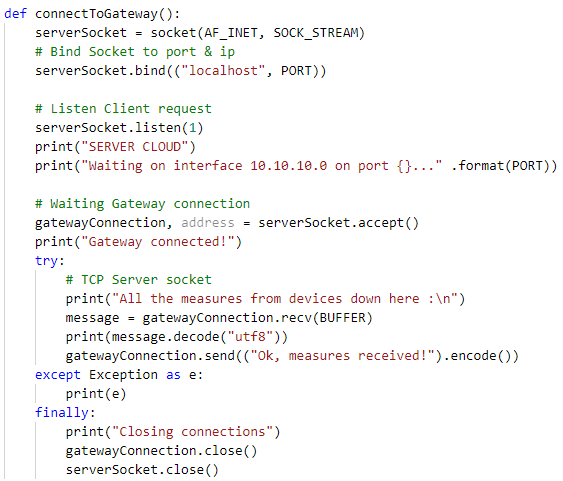
\includegraphics[width=\textwidth]{img/cloud.png}}
	\end{figure}
	
	\chapter{Spiegazione dettagliata del Funzionamento}
	
	\begin{itemize}
		\item\textbf{ 1° Passo}: Avviamo il Gateway e il Cloud Server che aspettano entrambi in ascolto sulla propria interfaccia che qualcuno gli invii dei dati
		\item \textbf{2° Passo}: Avviamo i 4 Device IoT che leggono le misure rilevate e le inviano al Gateway, indicando anche il tempo impiegato per la connessione UDP e il buffer utilizzato
		\item \textbf{3° Passo}: Una volta fatti partire tutti i moduli pyton, il Gateway riceverà le misure dei quattro Device IoT (è presente un controllo che non permette ai Device di mandare più volte la misura lo stesso giorno, in modo da poter leggere tutti e quattro i socket). Alla fine il Gateway stesso procederà a inviare al Cloud Server, tramite una connessione TCP, tutte le misure indicando anche il tempo e la dimensione del Buffer.
	\end{itemize}
	
	

\end{document}